\newcommand{\nazov}{\textit{Výkonové spínací tranzistory} }
\newcommand{\typprace}{diplomov}


%%%%%%%%%%%%%%%%%%%%%%%%%%
%%	TITULNY LIST	%%
%%%%%%%%%%%%%%%%%%%%%%%%%%
\thispagestyle{empty}

%\begin{minipage}[t]{.16\textwidth}
%	\includegraphics[width=.8\textwidth]{kapitoly/logoVUT} \ \
%\end{minipage}
%\begin{minipage}[t][t]{.5\textwidth}
%	alkalkja
%
%	a,a,a,a,
%	llkfdj
%
%	sdlojsdlj
%
%	slkdldsjk
%\end{minipage}

%\noindent
%\begin{tabular}{p{.16\textwidth}  p{.8\textwidth} }
%	\vspace{48pt}\includegraphics[width=.16\textwidth]{kapitoly/logoVUT} & 
%	\large\textsc{Vysoké učení technické v~Brně} \newline \footnotesize{} \newline
%	\normalsize\textsc{Brno University of Technology}
%\end{tabular}
%\par

%%\vspace{6pt}
%\noindent
%\begin{tabular}{p{.16\textwidth}  p{.8\textwidth} }
%	\vspace{56pt}\includegraphics[width=.16\textwidth]{kapitoly/logoFEKT} & 
%	\normalsize\textsc{Fakulta elektrotechniky a komunikačních technologií} \newline
%	\normalsize\textsc{Ústav výkonové elektrotechniky a elektroniky} \newline
%	\newline 
%	\small\textsc{Faculty of Electrical Engineering and Communication} \newline
%	\small\textsc{Department of Power Electrical and Electronic Engineering}
%\end{tabular}
%\par

%\vspace{96pt}
%%\centering
%\begin{center}
%\LARGE\textsc{\textbf{Výkonové spínací tranzistory\\}}
%\vspace{12pt}
%\large\textsc{Power Switching Transistors}
%\end{center}
%\par
%
%\vspace{120pt}
%\noindent
%\begin{tabular}{p{.40\textwidth}  p{.60\textwidth} }
%	\large\textsc{Semestrální práce}\newline
%	\normalsize\textsc{Semestral Thesis}\\
%	\\
%	\large\textsc{Autor práce}\newline
%	\normalsize\textsc{Author}		&	\normalsize Bc. \textsc{Ján Mikláš}\\
%	\\
%	\large\textsc{Vedoucí práce}\newline
%	\normalsize\textsc{Supervisor}		&	\normalsize doc. Dr. Ing. \textsc{Miroslav Patočka}\\
%	\\
%	\\
%	\normalsize\textsc{Brno 2016}
%\end{tabular}
%\par
%\normalsize

\includegraphics[height=\textheight]{TitulniList_black-crop}

\newpage\thispagestyle{empty}\mbox{}
% cista strana - kvoli obojstrannej tlaci a zadaniu


\newpage
%%%%%%%%%%%%%%%%%%%%%%%%%%%%%%%%%%%%%%%%%%%%%%%%%%%%%%%%ť

%\thispagestyle{empty}
%includegraphics[height=\textheight]{kapitoly/titulnylist-crop}
%\newpage
\thispagestyle{empty}
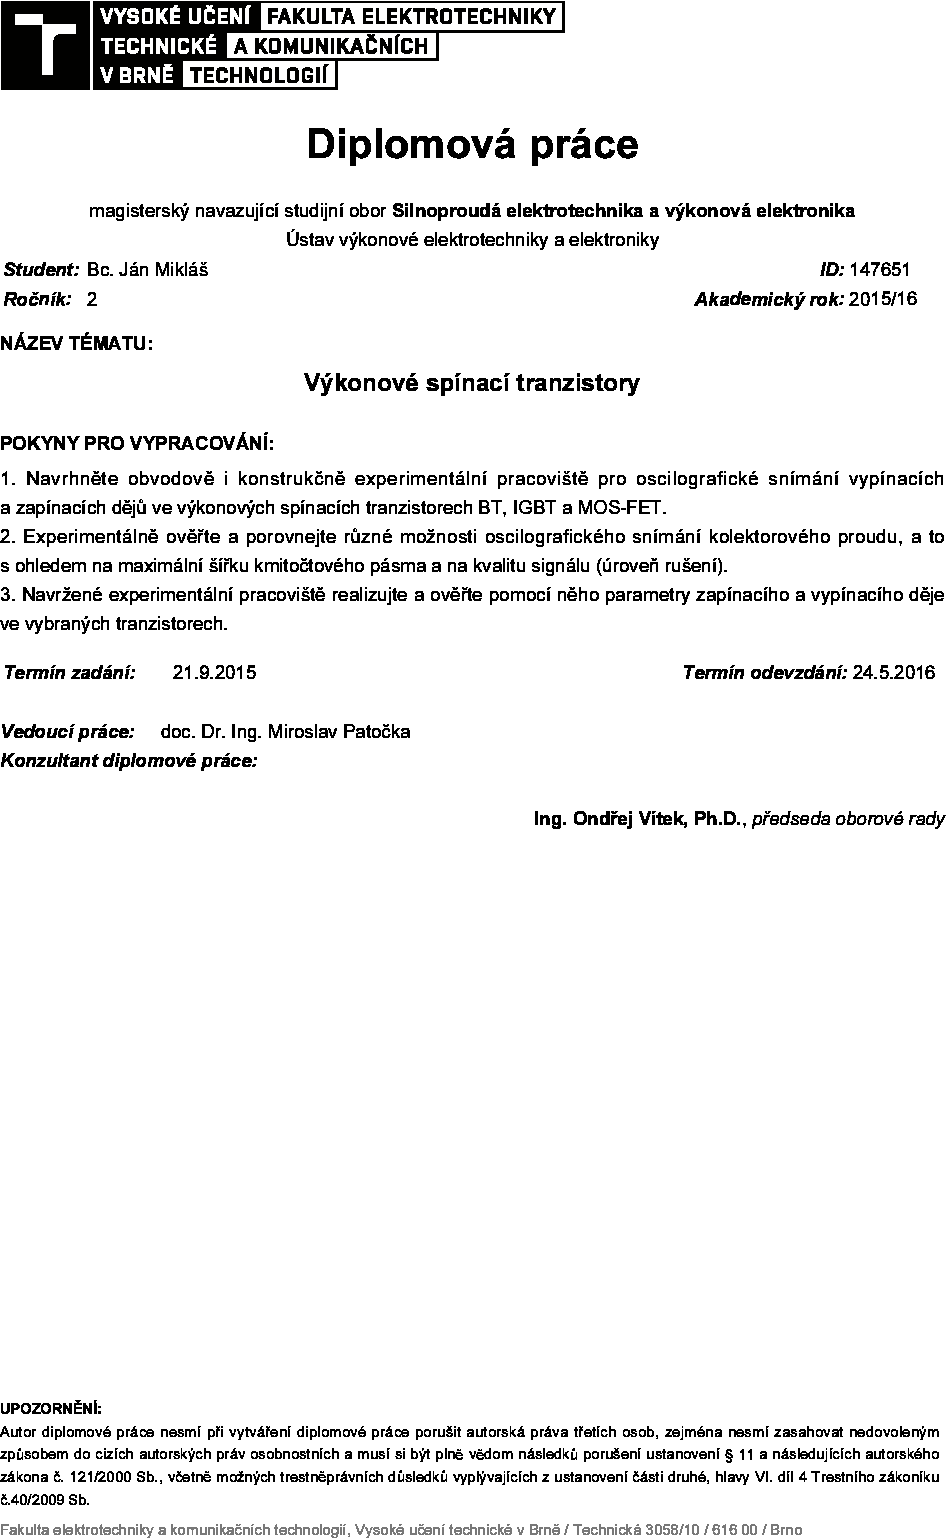
\includegraphics[width=\textwidth]{zadanieDP-crop}




\newpage\thispagestyle{empty}\mbox{}
% cista strana - kvoli obojstrannej tlaci a zadaniu

\newpage\thispagestyle{empty}\mbox{}


\newpage
\thispagestyle{empty}
\section*{Kľúčové slová}
výkonové spínacie tranzistory, spínacie straty, priebehy zapínacieho deja, priebehy vypínacieho deja, meranie spínacích strát, snímanie prúdu, simulačný model spínacieho tranzistora
\vspace{30mm}
\section*{Keywords}
power switching transistor, switching loss, turn on waveform, turn off waveform, switching loss measurements, current sensor, switching transistor simulation model

\newpage
\thispagestyle{empty}
\section*{Abstrakt}
V práci sú popísané predpoklady meraní spínacích strát, ktoré boli vykonané v rámci práce a je navrhnutý napäťový medziobvod a budič výkonových tranzistorov.

Nasleduje odvodenie funkcie aproximujúcej priebeh vodivosti $g_{CE} = \frac{i_C}{u_{CE}}$, ukážky simulácie spínacích dejov pomocou tejto vodivosti a pojednanie o zmeraných priebehoch.

\paragraph{}


\section*{Abstract}
In this thesis, prerequisities for a switching loss measurements  are established as well as designing of DC-bus and the base/gate driver for the power transistors; followed by derivation of  mathematical approximation of transistor conductivity $g_{CE} = \frac{i_C}{u_{CE}}$, circuit simulation using $g_{CE}$ as a transistor model and a discussion of measured waveforms.



\newpage
\thispagestyle{empty}
\section*{Bibliografická citácia}
MIKLÁŠ, J. \nazov. Brno: Vysoké učení technické v~Brně, Fakulta elektrotechniky a komunikačních technologií, 2016. \pageref{LastPage} s. Vedoucí diplomové práce doc. Dr. Ing. Miroslav Patočka.

\newpage
\thispagestyle{empty}
\section*{Prehlásenie}

Prehlasujem, že svoju diplomovú~prácu na tému \nazov som vypracoval samostatne pod vedením vedúceho \typprace ej práce a s~použitím odbornej literatúry a ďalších informačných zdrojov, ktoré sú všetky citované a uvedené v~zozname literatúry na konci práce.
Ako autor uvedenej \typprace ej práce ďalej prehlasujem, že v~súvislosti s~vytvorením tejto práce som neporušil autorské práva tretích osôb, predovšetkým som nezasiahol nedovoleným spôsobom do cudzích autorských práv osobnostných a som si plne vedomý následkov porušenia ustanovenia § 11 a nasledujúcich autorského zákona č. 121/2000 Sb., včítane  možných
trestnoprávnych dôsledkov vyplývajúcich z~ustanovenia § 152 trestného zákona č. 140/1961 Sb.

\vspace{2cm}
V~Brne dňa \ldots\ldots\ldots\ldots\ldots \hspace{30mm}Podpis \ldots\ldots\ldots\ldots\ldots
%\vspace{5cm}



\newpage\thispagestyle{empty}\mbox{}

\section*{Poďakovanie}
Ďakujem v prvom rade vedúcemu práce doc. Dr. Ing. Miroslavovi Patočkovi za vecné, presné a účinné rady a vedenie v práci. Tiež ďakujem Ing. Petrovi Procházkovi, Ph.D. za ochotu a spoluprácu.
